\documentclass{classrep}
\usepackage[utf8]{inputenc}
\usepackage{color}
\usepackage{amsmath}
\usepackage{dirtytalk}
\usepackage{latexsym}
\usepackage{multirow}
\usepackage{graphicx}
\usepackage{float}
\newtheorem{exmp}{Przykład}[section]
\studycycle{Informatyka, studia STACJONARNE, I st.}
\coursesemester{VI}

\coursename{Komputerowe systemy rozpoznawania}
\courseyear{2020/2021}

\courseteacher{prof. dr hab. inż. Adam Niewiadomski}
\coursegroup{poniedziałek, 12:00}

\author{
  \studentinfo{Hubert Gawłowski}{224298} \and
  \studentinfo{Kamil Kiszko-Zgierski}{224328} }

\title{Projekt 1. Klasyfikacja dokumentów tekstowych}

\begin{document}
\maketitle

\section{Cel projektu}

Celem zadania jest zaimplementowanie algorytmu $k$-NN w technologii Java na potrzeby klasyfikacji tekstów
oraz zbadanie wpływu wybranych cech liczbowych i tekstowych na skuteczność powyższej metody. W wyniku działania algorytmu teksty zostaną przyporządkowane do krajów, z jakich pochodzą.
Badanie zostanie przeprowadzone na podstawie artykułów prasowych z agencji prasowej Reuters, które to pochodzą z 1987 roku, wszystkie teksty napisane są w języku angielskim, a przy klasyfikacji pod uwagę będą brane artykuły, które pochodzą z następujących krajów: Republika Federalna Niemiec, USA, Francja, Wielka Brytania, Kanada, Japonia.  \\


\section{Klasyfikacja nadzorowana metodą $k$-NN}
Algorytm $k$-NN (od angielskich słów nearest neighbour - najbliższy sąsiad) to algorytm, 
którego działanie polega na przyporządkowaniu obiektu poddanego rozpoznawaniu do jednej z klas.
 Do wykorzystania tego algorytmu niezbędny jest zestaw klas, do których może należeć obiekt, zbiór danych uczących oraz rozpoznawany obiekt.
Metoda $k$-NN należy do grupy metod minimalnoodległościowych, ponieważ o zaklasyfikowaniu obiektu 
do danej klasy decyduje najmniejsza odległość (zgodna z przyjętą metryką), pomiędzy rozpoznawanym obiektem oraz k-obiektami z ciągu uczącego. 
Wyszukiwanie najmniejszej odległości pomiędzy obiektami można przedstawić za pomocą wzoru ogólnego:
\begin{gather}
\rho(x, x ^ {i, k})= \min_{x^\mu \in U^i}(x, x^\mu)
\end{gather}
\indent gdzie $\rho$ to wybrana metryka, $U^i$ oznacza ciąg uczący, $x^{i, k}$ jest elementem zbioru $U^i$, a rozpoznawany obiekt to x \cite{tadeusiewicz90}.\\
\indent Skuteczność algorytmu $k$-NN  mierzona jest na podstawie odsetka poprawnych przyporządkowań obiektów do odpowiadających im klas. 


\subsection{Ekstrakcja cech, wektory cech}

Pierwszym etapem, który należy wykonać w procesie rozpoznawania tekstów jest wyodrębnienie takich cech, 
aby jak najlepiej określały ich charakterystykę.Wszystkie artykuły są napisane w tym samym języku oraz w tej samej formie stylistycznej, 
dlatego w trakcie analizy skupiliśmy się na cechach liczbowych oraz tekstowych. Mając to na uwadzę, dokonaliśmy ekstrakcji poniższych cech:
\begin{enumerate}
    \item Zapis cyfr - za pomocą analizy ciągu cyfr otrzymamy informacje o np. numerach telefonicznych, które to są charakterystyczne dla omawianego kraju. Z pomocą symboli matematycznych ceche tą możemy zapisać następująco:  
    \begin{equation}
        c_1 = \frac{|{s: s \in N \land s \in P_k}|}{w}
    \end{equation}
    gdzie $N$- zbiór ciągów cyfr znalezionych w dokumencie, $P$ - zbiór charakterystycznych ciągów cyfr dla danego kraju k, $w$ - waga przez jaką należy podzielić otrzymaną cechę.\\
    Wzór ten zastosujemy dla każdego z rozpatrywanych krajów i dzięki porównaniu otrzymanych wyników uzyskamy informacje do której grupy, na podstawie tej cechy, sklasyfikować dany dokument. \\
    \begin{exmp}Fragment artykułu pt. "Offers USA direct service in Denmark" \cite{reuters}\\
    \say{[...]The service allows callers in Denmark to reach an ATT
operator in the United States by dialing a single telephone
number, 0430-0010, ATT said.[...]}. \\
    \end{exmp}
Z powyższego fragmentu możemy wyodrębnić ciąg cyfr 0430-0010 i na jego podstawie sklasyfikować, do jakiej etykiety kraju możemy zaklasyfikować dany artykuł. Numery telefonów z różnych krajów mogą być rozpoznane na podstawie np. numeru kierunkowego, ich długości czy też formatu zapisu. \\
    \item Waluty - wyciągnięcie z tekstów nazw najczęsciej używanych walut. Każdy z krajów posługuje się inną walutą \footnote{Omawiane artykuły pochodzą z lat 80, kiedy we Francji i w Niemczech obowiązywała inna waluta (odpowiednio frank francuski i marka niemiecka). Kraje te przyjęły wspólną walutę, tj. euro dopiero w 2002 roku}, dlatego jest to cecha, która jasno charakteryzuje nam wybrane kraje. Wzory do tej cechy będą prezentowały się nasepująco:
	\begin{gather}
	    c_2' = d_{t}(M)
	\end{gather} 
    \indent gdzie $d_{t}$ jest funkcją wyznaczającą t najczęściej występujących słów w danym zbiorze, M to zbiór znalezionych w artykule słów oznaczających waluty.
    \begin{gather}
        c_2 = g_k(c_2')
    \end{gather}
    \indent gdzie $g_k$ jest funkcją przyporządkowującą wyznaczone słowa do poszczególnego kraju k.\\
    W wyniku porównania otrzymanych dla każdego kraju wartości będziemy mogli stwierdzić do którego kraju, na podstawie tej cechy, można przyporządkować podany tekst.\\
    
    \begin{exmp}Fragment artykułu pt. "Maxtor agrees to acquire U.S. design" \cite{reuters}\\ 
    \say{[...]They said the arrangement, which is subject to a number of
    conditions including U.S. Design shareholder approval, calls
    for Maxtor to issue 12 mln dlrs worth of its own common stock
    in exchange for all of U.S. Design.[...]}. \\
    \end{exmp}
    W powyższym fragmencie została wymieniona waluta o nazwie dolar ("dlrs"). Mimo, że najbardziej popularnym dolarem jest dolar amerykański, natomiast na świecie jest jeszcze wiele innych walut, których pierwszym członem jest słowo "dolar", np. dolar kanadyjski, dolar australijski. Ten fakt należy również wziąć pod uwagę w momencie wyznaczania zbiorów rozmytych. Z podanego fragmentu wynika także, że aby w pełni skorzystać z tej cechy, należy uwzględnić nie tylko pełne nazwy walut, ale również ich skróty, które również się pojawiają w artykułach. \\
    \item Częstość występowania dat - zliczenie, jak często w podanych tekstach występują elementy określające czas. Wydaje się, że ich częstość będzie się różnić w zależności od pochodzenia tekstu. Powyższą cechę można przedstawić następująco:
    \begin{equation}
        c_3 = \frac{|{s: s \in D \land s \in A}|}{|A|}
    \end{equation}
    gdzie $D$ - zbiór słów oznaczających daty, $A$ - zbiór wszystkich słów z artykułu. \\
    \begin{exmp} Fragment artykułu pt. "USDA comments on export sales"  \cite{reuters} \\
    \say{[...]  In comments on its Export Sales Report, the department said
    sales of 1.0 mln tonnes to the USSR -- previously reported
    under the daily reporting system -- were the first sales for
    delivery to the USSR under the fourth year of the U.S.-USSR
    Grains Supply Agreement, which began October 1.
    [...]
        Egypt, Japan and Iraq were the major wheat buyers for
    delivery in the current year, while sales to China decreased by
    30,000 tonnes for the current season, but increased by 90,000
    tonnes for the 1987/88 season, which begins June 1. [...]}. \\
    \end{exmp}W przytoczonym fragmencie zapis daty został wykorzystany 3 razy ("October 1", "1987/88", "June 1"). Wobec tego, uważamy, że opisywana cecha będzie korzystnie wpływać na proces klasyfikacji tekstów. \\

    \item Format zapisu dat - w zależności od kraju format zapisu dat różni się. Cechę tą zapisać można za pomocą wzorów:
    \begin{gather}
        c_4' = f(B)
    \end{gather}
    \indent gdzie f - funkcja wyznaczająca zapis datowy z podanego zbioru, B - zbiór wszystkich wyrażeń znajdujących się w artykule (wyrażenie traktujemy jako połączenie minimum dwóch słów).
    \begin{gather}
        c_4 = t_k(c_4')
    \end{gather}
    \indent gdzie $t_k$ jest funkcją przyporządkowującą wyznaczone wyrażenia do poszczególnego kraju k.\\
    Jako, że w kilku krajach stosowany jest ten sam zapis datowy, funkcja ta może (a wręcz jest to bardzo prawdopodobne) zwrócić taką samą wartość dla kilku krajów. W wyniku porównania otrzymanych dla każdego kraju wartości będziemy mogli stwierdzić do którego kraju (bądź kilku krajów z równym prawdopodobiństwem), na podstawie tej cechy, można przyporządkować podany tekst. 
    \\
    
    \begin{exmp} Fragment artykułu pt. "Software services extends warrants" \cite{reuters} \\ \say{[...]Software Services of America
    Inc said its board has extended the expiration date of its
    warrants until August 31 from April 30.[...]}\\
    \end{exmp} Daty występujące w tym fragmencie ("August 31" i "April 30") są zapisane w formacie: miesiąc dzień. Uważamy, że w zależności od tego, z jakiego kraju pochodzi artykuł format zapisu dat może się różnić. \\
    \item Ogólna liczba słów - zliczenie wszystkich słów występujących w tekście. Uważamy, że w zależności od tego, jakiego kraju tekst dotyczy, ich długość może być różna. Liczbę wyrazów znajdujących się w tekście można przedstawić następująco:
    \begin{equation}
        c_5 = |A|
    \end{equation}
    gdzie $A$ - zbiór wszystkich słów z artykułu. \\
    \item Częstość słów rozpoczynających się wielką literą - słowa takie będą oznaczały najczęściej  nazwy własne np. imiona, nazwiska, nazwy budynków lub będą to rozwinięcia skrótów. Pisząc o jednym kraju może być używane więcej takich słów, 
	a o innych mniej. Z tej grupy wykluczymy jednak wyrazy składające się wyłącznie z wielkich liter (o których mowa będzie w punkcie następnym) oraz słowa pisane z wielkiej litery z uwagi na początek zdania. Aby odróżnić wielkie litery od małych, trzeba na początku dokonać odwzorowania liter w słowie na kody ASCII i następnie sprawdzić, czy odpowiedni kod ASCII znajduje się w przedziale od 65 do 90. W postaci wzoru wygląda to następująco:
	\begin{equation}
	f(l) = \begin{cases} 1 &\mbox{ jeśli }  l\in<65,90> \\ 0 & \mbox{ jeśli } l\notin<65,90> \end{cases}
	\end{equation}
	gdzie l oznacza pojedyńczy znak zapisany za pomocą kodu ASCII, a funkcja f(l) zwraca 1 dla liter zapisanych wielką literą, a 0 dla pozostałych znaków.
	Natomiast w celu obliczenia częstości słów rozpoczynających się wielką literą należy skorzystać z poniższego wzoru: 
	\begin{equation}
        c_6 = \frac{|{s: s \in Z \land s \notin W \land s \notin M}|}{|A|}
    \end{equation}
    gdzie $Z$ - zbiór słów, rozpoczynających się w arrtykule wielką literą, $A$ - zbiór wszystkich słów z artykułu, $W$ - zbiór słów, pisanych w artykule wielkimi literami, $M$ - zbiór słów, które rozpoczynają w artykule zdania. \\
	\begin{exmp}Fragment artykułu pt. "U.S. Auto Union will fight to stop job/wage cuts" \cite{reuters}\\
	\say{[...]The United Auto Workers union (UAW)
    vowed to fight wage and job cuts in a round of labour talks
    starting in July that cover nearly 500,000 workers at General
    Motors Corp and Ford Motor Co[...]}. \\
    \end{exmp}
    W tym krótkim fragmencie występuje aż 9 słów rozpoczynających się wielką literą, jednocześnie nie będących pierwszym słowem w zdaniu oraz nie będących słowem składających się tylko z wielkich liter. Słowa te są w tym fragmencie związane z nazwami własnymi oraz nazwą miesiąca. Uważamy, że przede wszystkim stosowanie nazw własnych może być związane z tym, z jakiego kraju pochodzi podany dokument. \\
    \item Częstość słów pisanych wielkymi literami - najczęściej będą to skróty. Uważamy, że w zależności od opisywanego kraju, ilość wykorzystywanych skrótów może się różnić. Do policzenia wystąpień słów zapisanych wielkimi literami należy wykorzystać poniższy wzór:
    \begin{equation}
        c_7 = \frac{|{s: s \in W}|}{|A|}
    \end{equation}
    gdzie $W$ - zbiór słów, pisanych w artykule wielkimi literami, $A$ - zbiór wszystkich słów z artykułu. \\ 
    \begin{exmp}Fragment artykułu pt."France approves large defence spending increase" \cite{reuters} \\
    \say {[...]The budget represents a six pct annual increase, starting next year, well above the 3.5 pct NATO recommends for members of its military command. France is a member of NATO but does
    not belong to its integrated military command.[...]} \\
    \end{exmp}
    W powyższym fragmencie skrót NATO(Organizacja Traktatu Północnoatlantyckiego) występuje 2 razy. Według nas, częstość występowania skrótów, w danym artykule może mieć związek z tym, jakiego kraju dotyczy tekst. \\
    \item Układ SI/imperialny - zdecydowanie częściej w artykułach z krajów anglojęzycznych będzie stosowany układ imperialny, natomiast w pozostałych - układ SI. 
    Wyliczenie liczby wystąpień jednostek w układzie SI można wyrazić następująco: 
     \begin{equation}
        c_8' = \frac{|{s: s \in S \land s \in A}|}{|A|}
    \end{equation}
    gdzie $S$ - zbiór słów oznaczających jednostki układu SI, $A$ - zbiór wszystkich słów z artykułu. \\
    Z kolei wzór do wyliczenia liczby wystąpień jednostek w układzie imperialnym przedstawia się w poniższy sposób:
    \begin{equation}
        c_8'' = \frac{|{s: s \in I \land s \in A}|}{|A|}
    \end{equation}
    gdzie $I$ - zbiór słów oznaczających jednostki układu imperialnego, $A$ - zbiór wszystkich słów z artykułu
    Jako opisywaną cechę zapisujemy różnicę wystąpień jednostek w układzie SI oraz imperialnym, czyli:
    \begin{equation}
        c_8 = {c_8'}-{c_8''}
    \end{equation} \\
    \begin{exmp}Fragment artykułu pt. "Sun in North Dakota oil find" \cite{reuters} \\
    \say{[...]flowed 660 barrels of oil and 581,000 cubic feet of natural gas per day through a 13/64 inch choke from depths of 13,188 to 13,204 feet.[...]}. \\
    \end{exmp}
    W powyższym tekście można zauważyć występowanie jednostkek z układu imperialnego, tj. cale(inch) i stopy(feet). Wobec tego, można przypuszczać, że tekst ten pochodzi z jednego z krajów anglojęzycznych. \\
    \item Częstość występowania cytatów - 
     kolejna cecha, która wydaje się różnić w zależności od kraju, o którym mowa w artykule. Liczba cytatów zostanie uzyskana w wyniku obliczenia liczby występowania słów, gdzie przedostatni znak to ',' lub '.', a ostatni '"'. Wyznaczenie  tej  cechy  można zaprezentować w postaci wzoru:
    \begin{equation}
        c_9 = \frac{|{s: s \in Y}|}{|A|}
    \end{equation}
    gdzie $Y$ - zbiór cytatów występujących w artykule, $A$ - zbiór wszystkich słów z artykułu. \\
    \begin{exmp}Fragment artykułu pt. "Hughes changes stance on merger after suit" \cite{reuters} \\
    \say{[...]"I think the merger is not going through," said Phil Pace,
    analyst at Kidder, Peabody and Co. He said the merger "lost a
    lot of its appeal" when the U.S. Department of Justice required
    that Baker sell off its Reed Tool Co operation.[...]}. \\
    \end{exmp}
    W podanym fragmencie cytat wystąpił 2 razy. Uważamy, że artykuły dotyczące różnych krajów będą też zawierały różną liczbę cytatów. \\

    \item Słowa kluczowe - sporządzone zostaną listy elementów identyfikujących każdy z krajów. Określenia te będą związane z elementami charakterystycznymi dla danego kraju. Możemy do nich zaliczyć nazwy geograficzne, znane osoby, nazwy firm itp.. Do wyznaczenia słów kluczowych należy skorzystać ze wzoru: 
    \begin{equation}
        c_{10} = \frac{|{s: s \in K \land s \in A}|}{|A|}
    \end{equation}
    gdzie $K$ - zbiór słów kluczowych, $A$ - zbiór wszystkich słów z artykułu. \\
    \begin{exmp}Fragment artykułu pt. "Currency futures to key off G-5, G-7 meetings" \cite{reuters} \\
    \say{[...]News of an agreement among G-5 and G-7
    finance ministers meeting in Washington this week will be key
    to the direction of currency futures at the International
    Monetary Market, but any such agreement will need to go beyond
    the Paris accord to stem the recent rise in futures, financial
    analysts said.[...]}. \\
    \end{exmp}
    Powyższy tekst zawiera 2 słowa kluczowe - Washington i Paris. Washington związane jest z USA, natomiast Paris z Francją. Chcąc przyporządkować ten fragment biorąc pod uwagę tylko i wyłącznie cechę związaną ze słowami kluczowymi zostałby dopasowany z równym prawdopodobieństwem do Francji lub USA. \\
    \item Najczęściej występujące słowa - wyodrębnienie z artykułów najczęściej występujących słów, z pominięciem słów znajdujących się na tzw. stopliście, tj. liście najczęściej używanych słów w języku angielskim \cite{coca_words}. Zabieg ten ma na celu podniesienie jakości klasyfikacji poprzez wyszukanie słów, które charakteryzują treść artykułu. Pominięcie tej operacji skutkowałoby niejednoznacznym zaklasyfikowaniem tekstów, co w konsekwencji obniżyłoby skuteczność algorytmu. 
	Wyznaczenie opisywanej cechy można przedstawić w postaci operacji na zbiorach:
	\begin{gather}
	c_{11}= d_{t}(A - S)
	\end{gather} 
	\indent gdzie $d_{t}$ jest funkcją wyznaczającą t najczęściej występujących słów w danym zbiorze, A to zbiór słów w artykule, 
	a S jest zbiorem słów znajdujących się na stopliście. \\
	\begin{exmp}
    Fragment artykułu pt. "Houston oil trust"  \cite{reuters} \\
    \say {[...] The most significant factor for the lack of a distribution
    this month is the establishment of additional special cost
    escrow accounts, the company said, adding, that there may be no
    cash distribution in other months or during the remainder of
    the year [...]} \\
    \end{exmp} 
    Dla powyższego przykładu załóżmy, że stoplista obejmuje 100 najczęściej używanych słów w języku angielskim. Stosując wzór (2) okazuje się, że najczęściej występującym charakterystycznym słowem jest distribution, które pojawiło się w tekście 3 razy. \\
\end{enumerate}
Ostatecznie, wektor wyekstrahowanych cech będzie się prezentował następująco: 
\begin{gather}
v = [c_{1}, c_{2}, c_{3}, c_{4}, c_{5}, c_{6}, c_{7}, c_{8}, c_{9}, c_{10}, c_{11}] 
\end{gather}

\subsection{Miary jakości klasyfikacji} 
Podczas procesu klasyfikacji niezbędne jest określenie jak skuteczna i jakościowa jest prowadzona klasyfikacja. W tym celu posłużyliśmy się tablicą(macierzą) pomyłek oraz miarami jakości klasyfikacji.\cite{tablica_pomylek} Macierz pomyłek zawiera ilość próbek przypisanej do poszczególnej grupy (prawdziwie pozytywna, fałszywie pozytywna, fałszywie negatywna, prawdziwie negatywna). Grupy te powstają poprzez zestawienie ze sobą klasy rzeczywistej oraz klasy predykowanej. Tablica pomyłek prezentuje się następująco: \\

\begin{table}[h]
    \centering
        \begin{tabular}{cc|p{30mm}|p{30mm}|p{30mm}|p{30mm}|l}
        \cline{3-4}
        & & \multicolumn{2}{ c| }{Klasa rzeczywista} \\ \cline{3-4}
        & & pozytywna & negatywna\\ \cline{1-4}
        \multicolumn{1}{ |c  }{\multirow{2}{*}{Klasa predykowana} } &
        \multicolumn{1}{ |c| }{pozytywna} & prawdziwie \newline pozytywna (TP) & fałszywie \newline pozytywna (FP) \\ \cline{2-4}
        \multicolumn{1}{ |c  }{}                        &
        \multicolumn{1}{ |c| }{negatywna} & fałszywie \newline negatywna (FN) & prawdziwie \newline negatywna (TN)     \\ \cline{1-4}
        \end{tabular}
    \caption{Tablica pomyłek}
\end{table}
 Zostały wykorzystane następujące miary jakości, które zostaną przedstawione wzorami, w których oznaczenia odnosić się będą do Tabeli 1:
\begin{itemize}
    \item Accuracy (dokładność) - miara, która oznacza dokładność całej klasyfikacji:
    \begin{equation}
        ACC = \frac{TP + TN}{L}
    \end{equation}
    \indent gdzie $L$ - liczba wszytskich sklasyfikowanych próbek
    \item Precision (precyzja) - miara oznaczająca jak często określoną klasę udało się zakwalifikować poprawnie:
    \begin{equation}
        PPV = \frac{TP}{TP+FP}
    \end{equation}
    \item Recall (czułość) - określa jak dużo wystąpień obiektów danej klasy zakwalifikowaliśmy do tejże klasy:
    \begin{equation}
        TPR = \frac{TP}{TP+FN}
    \end{equation}
    \item F1 - miara stanowiąca średnią harmoniczną z miar Precision i Recall \cite{f1}:
    \begin{equation}
        F_1 = 2\cdot \frac{PPV \cdot TPR}{PPV+TPR}
    \end{equation}
\end{itemize}
Dla przykładu obliczmy miary jakości dla poniższej tabeli:

\begin{table}[h]
    \centering
        \begin{tabular}{cc|p{30mm}|p{30mm}|p{30mm}|p{30mm}|l}
        \cline{3-4}
        & & \multicolumn{2}{ c| }{Klasa rzeczywista} \\ \cline{3-4}
        & & $Japonia$ & $\sim Japonia$\\ \cline{1-4}
        \multicolumn{1}{ |c  }{\multirow{2}{*}{Klasa predykowana} } &
        \multicolumn{1}{ |c| }{$Japonia$} & 56 & 12 \\ \cline{2-4}
        \multicolumn{1}{ |c  }{}                        &
        \multicolumn{1}{ |c| }{$\sim Japonia$} & 17 & 36    \\ \cline{1-4}
        \end{tabular}
    \caption{Tablica pomyłek z przykładowymi danymi}
\end{table}
\begin{equation}
    ACC = \frac{56+36}{121} = 0,76
\end{equation}
\begin{equation}
    PPV = \frac{56}{56+12} = 0,82
\end{equation}
\begin{equation}
    TPR = \frac{56}{56+17} = 0,77
\end{equation}
\begin{equation}
    F_1 = 2 \cdot \frac{0,82 \cdot 0,77}{0,82+0,77} = 0,79
\end{equation}



\section{Klasyfikacja z użyciem metryk i miar podobieństwa tekstów}
 Jak już zostało wspomniane w rozdziale 2., algorytm k-NN należy do grupy algorytmów minimalnoodległościowych. Aby zaimplementować jego działanie niezbędna jest zatem metryka, która pozwoli w transparentny sposób wyznaczyć odległości pomiędzy wektorami cech. Z tego względu, w ramach badań zostaną wykorzystane trzy poniższe rodzaje metryk:
 \begin{itemize}
    \item Euklidesowa - aby obliczyć odległość pomiędzy dwoma wektorami cech należy obliczyć pierwiastek z sumy kwadratów różnic wszystkich kolejnych cech obu wektorów. Wzór opisujący metrykę Euklidesową wygląda następująco \cite{tadeusiewicz90}:
    \begin{equation}
        \rho_{1}(c^\mu, c^\eta) = \sqrt{\sum_{\nu=1}^{n}(c_{\nu}^\mu - c_{\nu}^\eta)^2}
    \end{equation}
    \indent ,gdzie $c^\mu$ oraz $c^\eta$ oznaczają wektory cech, natomiast n jest to liczba cech, a $\nu$ to numer cechy \\
    \begin{exmp} Obliczanie metryki Euklidesowej  \\
        Dajmy dwa wektory cech:
        \begin{equation}
            c^\mu = [1, 2, 3]
        \end{equation}
        \begin{equation}
            c^\eta = [-2, -3, -4]
        \end{equation}
        Wynik obliczenia metryki euklidesowej przedstawia się następująco:
        \begin{equation}
            \rho_{1}(c^\mu, c^\eta) = \sqrt{(1 - (-2))^2 + (2 - (-3))^2 + (3 - (-4))^2}
        \end{equation}
        \begin{equation}
            \rho_{1}(c^\mu, c^\eta) = \sqrt{3^2 + 5^2 + 7^2}
        \end{equation}
        \begin{equation}
            \rho_{1}(c^\mu, c^\eta) \approx 9.11
        \end{equation} \\
    \end{exmp}
    \item uliczna - w celu obliczenia metryki ulicznej należy obliczyć sumę wartości bezwzględnych z różnic pomiędzy kolejnymi cechami z obu wektorów. Wzór opisujący metrykę uliczną wygląda następująco \cite{tadeusiewicz90}:
    \begin{equation}
        \rho_{2}(c^\mu, c^\eta) = \sum_{\nu=1}^{n}|c_{\nu}^\mu - c_{\nu}^\eta|
    \end{equation}
    \begin{exmp} Obliczanie metryki ulicznej

        Dajmy dwa wektory cech:
        \begin{equation}
            c^\mu = [3, 5, 8]
        \end{equation}
        \begin{equation}
            c^\eta = [-2, 0, 10]
        \end{equation}
        Wynik obliczenia metryki ulicznej przedstawia się następująco:
        \begin{equation}
            \rho_{2}(c^\mu, c^\eta) = |3 - (-2)| + |5 - 0| + |8 - 10| 
        \end{equation}
        \begin{equation}
            \rho_{2}(c^\mu, c^\eta) = 12
        \end{equation} \\
    \end{exmp}
    \item Czebyszewa - aby obliczyć metrykę Czebyszewa należy wyznaczyć maksymalną wartość bezwzględną z różnic pomiędzy kolejnymi cechami z obu wektorów. Wzór opisujący tę metrykę wygląda następująco \cite{tadeusiewicz90}:
    \begin{equation}
        \rho_{3}(c^\mu, c^\eta) = \max\limits_{1 \leq \nu \leq n}
        |c_{\nu}^\mu - c_{\nu}^\eta|
    \end{equation}
    \begin{exmp} Wykorzystanie metryki Czebyszewa  \\
        Dajmy dwa wektory cech:
        \begin{equation}
            c^\mu = [6, 3, 5, -1]
        \end{equation}
        \begin{equation}
            c^\eta = [3, 4, 1, 9]
        \end{equation}
        Wynik obliczenia metryki ulicznej przedstawia się następująco:
        \begin{equation}
            \rho_{3}(c^\mu, c^\eta) = max{|6 - 3|, |3 - 4|, |5 - 1|, |-1 - 9|}
        \end{equation}
        \begin{equation}
            \rho_{3}(c^\mu, c^\eta) = 10
        \end{equation} \\
    \end{exmp}
\end{itemize}

Nie wszystkie wartości w wektorze cech są od razu zapisane w formie liczbowej, niektóre z nich są w postaci tekstowej. W tym celu należy zaimplemetować miarę podobieństwa tekstów, która zamieni elementy wektora cech z postaci tekstowej na postać liczbową. W naszej aplikacji w tym celu wykorzystaliśmy Uogólnioną miarę n-gramów.\cite{wyklad} Zwykła metoda n-gramów określa podobieństwo łańcuchów tekstowych s1, s2 w oparciu o ilość wspólnych podciągów n-elementowych, (np. dla n=3 badamy podobieństwo słów w oparciu o podciągi 3-literowe). Zastosowana przez nas miara jest dokładniejsza, jednak bardziej kosztowna obliczeniowo - sprawdza ona podciągi różnej długości, od jedno- do N-elementowych, gdzie N jest długością słowa. Wyraża się ona wzorem:\\
\begin{equation}
    \mu_N(s_1,s_2) = \frac{2}{N^2+N}\sum_{i=1}^{N(s_1)}\sum_{j=1}^{N(s_1)-i+1}h(i,j)\
\end{equation}
 gdzie
 \newline$h(i,j) = 1$ jeśli $i$-elementowy podciąg w słowie $s_1$ zaczynający się od $j$-tej pozycji w słowie $s_1$ pojawia się przynajmniej raz w słowie $s_2$ (inaczej $h(i,j)=0$);
 \newline$N(s_1), N(s_2)$ - ilość liter w słowach $s_1$ i $s_2$;
 \newline $N = max\{N(s_1), N(s_2)\}$
 \newline $\frac{N^2+N}{2}$ - ilość możliwych podciągów od 1-elementowych do N-elementowych w słowie o długości N.



\section{Budowa aplikacji}
\subsection{Diagramy UML}
Nasza aplikacja będzie się składać z 4 modułów: moduł ekstrakcji, moduł klasyfikatora, moduł DAO (zarządzanie wczytywaniem danych z plików) oraz moduł interfejsu graficznego.

\indent Moduł ekstrakcji będzie odpowiedzialny za odwzorowanie tekstu na wektor cech. Wektor cech zaimplementowany zostanie z wykorzystaniem klasy FeaturesVector. W klasie FeaturesVector znajduje się 11 pól, każde oznaczające jedną z cech, które zostały przez nas wybrane i przedstawione w sekcji 2. Dla każdej cechy stworzona została odpowiadająca klasa. Każda z klas, która reprezentuje cechę, implementuje interfejs: dla cech liczbowych jest to interfejs NumericFeature, natomiast dla cech tekstowych jest n to interfejs TextFeature.
Oba interfejsy mają metodę extract(Article article), różnica polega na zwracanej wartości. W pierwszym przypadku jest to liczba typu integer (oznaczająca obliczoną liczbę np. słów w tekście), zaś w drugim przypadku jest to lista ciągów znaków (oznaczająca wyznaczoną, znalezioną listę wyrazów, które spełniają warunki danej klasy).
\\
\begin{figure}[H]
    \centering
    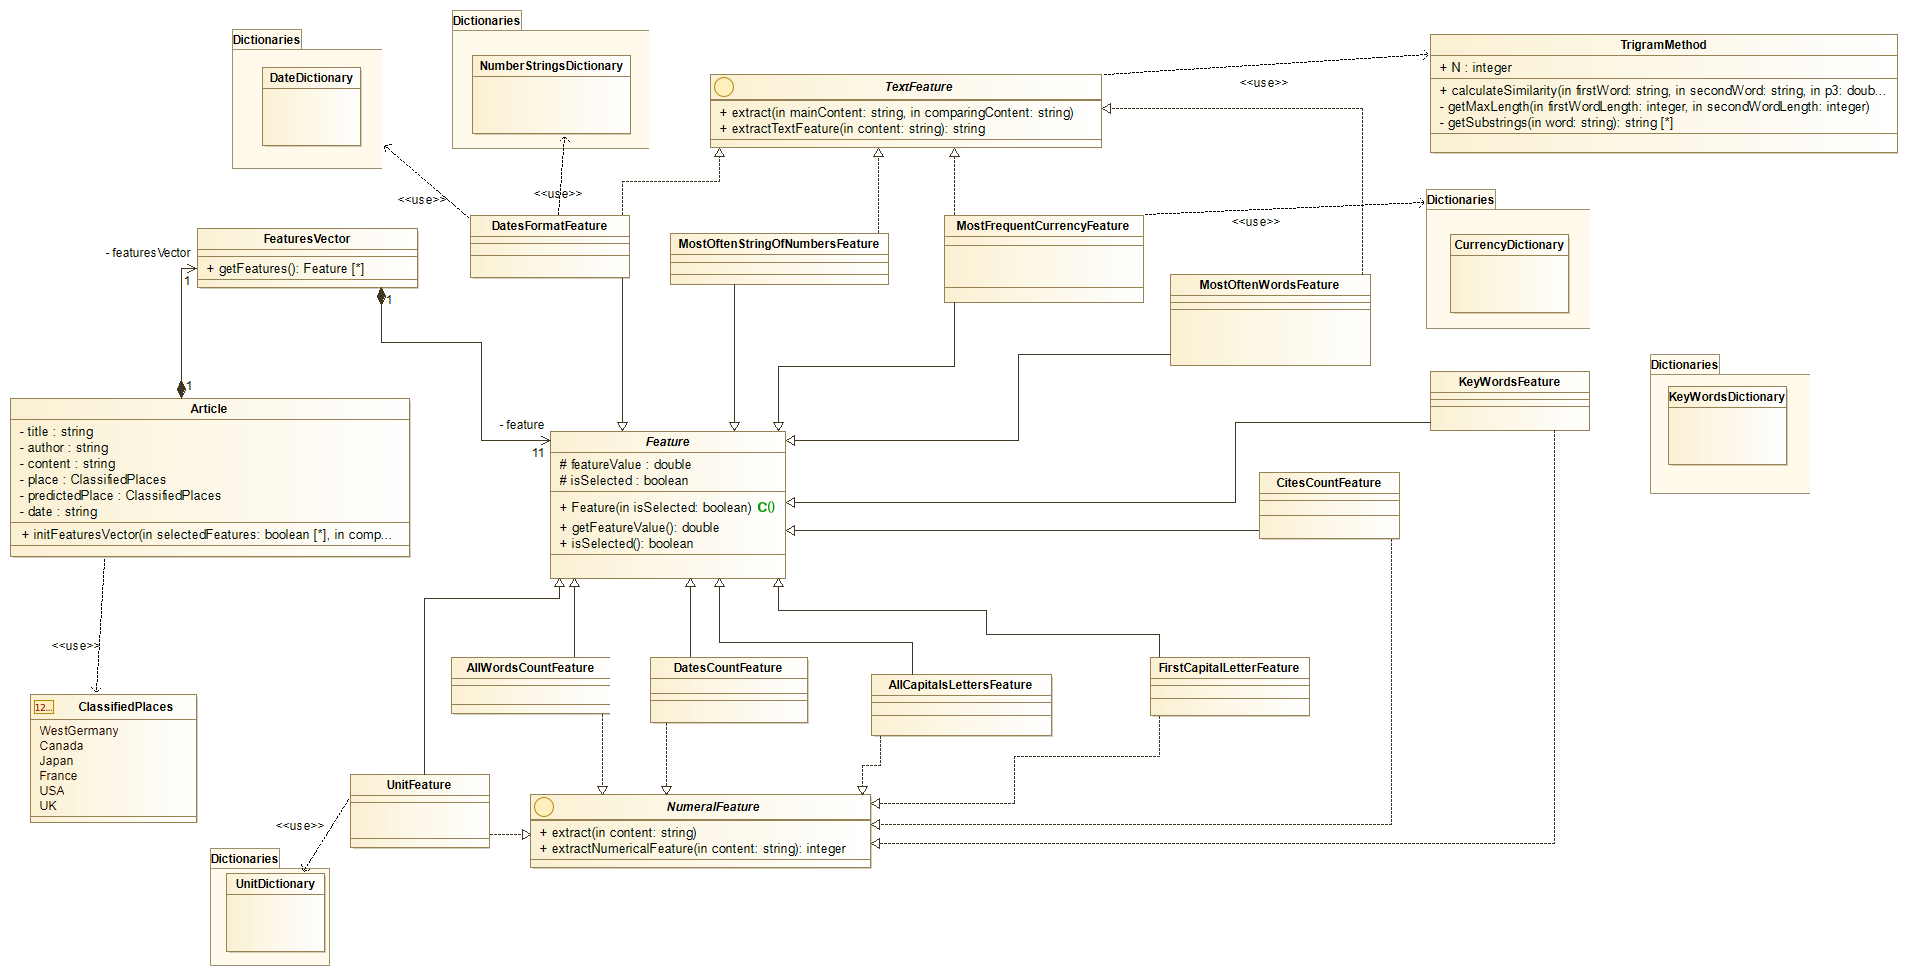
\includegraphics[width=15cm, height=10cm]{modul_ekstrakcji.png}
    \caption{Diagram UML dla modułu ekstrakcji}
\end{figure}


\indent Moduł klasyfikatora będzie odpowiedzialny za klasyfikację artykułów do odpowiednich etykiet places przy pomocy algorytmu kNN. Z tego względu powstanie klasa KnnClassifier, której zadaniem będzie sklasyfikowanie artykułu z wykorzystaniem jednej z trzech metryk, tj. metryki Czebyszewa, metryki ulicznej (Manhattan) lub metryki euklidesowej. W tym celu powstały cztery klasy: klasa Metric jest to klasa abstrakcyjna, natomiast klasy EuclideanMetric, ChebyshevMetric oraz ManhattanMetric są klasami dziedziczącymi. Poza metryką, niezbędne do klasyfikacji są paramtery: liczba najbliższych sąsiadów (kNeighbours) oraz stosunek liczby artykułów w części treningowej do części testowej. Do wykorzystania klasy KnnClassifier niezbędny jest moduł ekstrakcji, ponieważ klasa KnnClassifier wykorzystuje klasę Artykuł oraz kategorie ClassifiedPlaces znajdujące się w typie enumerate. \\
\begin{figure}[H]
    \centering
    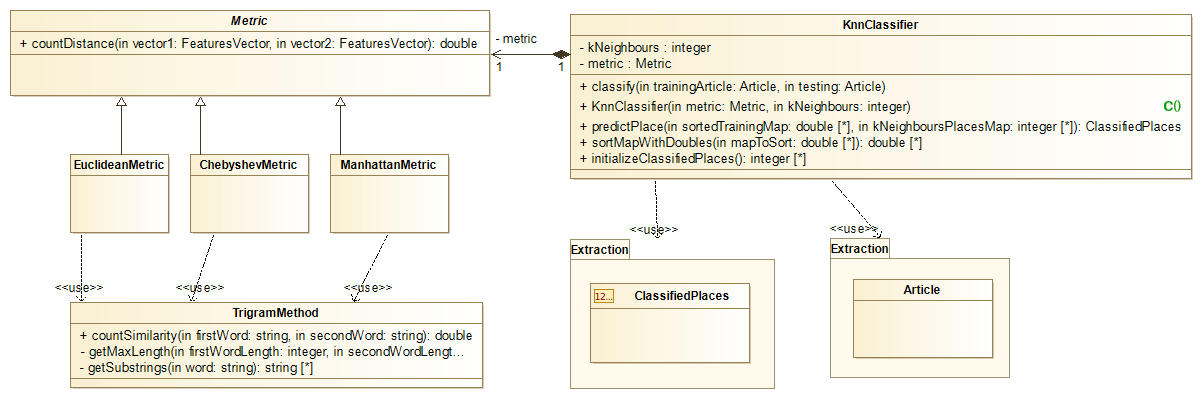
\includegraphics[width=15cm, height=10cm]{modul_klasyfikatora.png}
    \caption{Diagram UML dla modułu klasyfikatora}
\end{figure}

\subsection{Prezentacja wyników, interfejs użytkownika}
Aplikacja została wykonana w technologii Java w wersji 11\cite{java_11} (najnowsza wersja LTS) przy wykorzystaniu Apache Maven w wersji 3.6.3\cite{maven}. Do stworzenia interfejsu graficznego posłużyliśmy biblioteką JavaFX w wersji 13\cite{javafx}. W celu uruchomienia aplikacji należy po zainstalowaniu Maven na własnym kpmputerze, z poziomu wiersza poleceń znajdując się w folderze głównym projektu wykonać polecenie: mvn install, a następnie z wiersza poleceń z poziomu modułu GUI wykonać polecenie: mvn clean javafx:run. Aplikacje można także uruchomić z poziomu IDE. Po uruchuomieniu aplikacji ukaże nam się interfejs użytkownika, w którym możemy wybrać jak ma zostać podzielony zbiór (w jakich proporcjach na część treningową i testową), wczytać pliki, w których znajdują się teksty do analizy, podać licbę k najbliższych sąsiadów dla klasyfiaktora $k$-NN, wybrać metrykę oraz zbiór cech wykorzystywanych w procesie klasyfikacji oraz wykonać klasyfikację. W efekcie ukażą nam się następujące informacje: liczba wczytanych plików, liczba artykułów podlegających klasyfikacji oraz rezultaty 4 miar podobieństwa - Accuracy, Precision, Recall i F1.
\\
\begin{figure}[H]
    \centering
    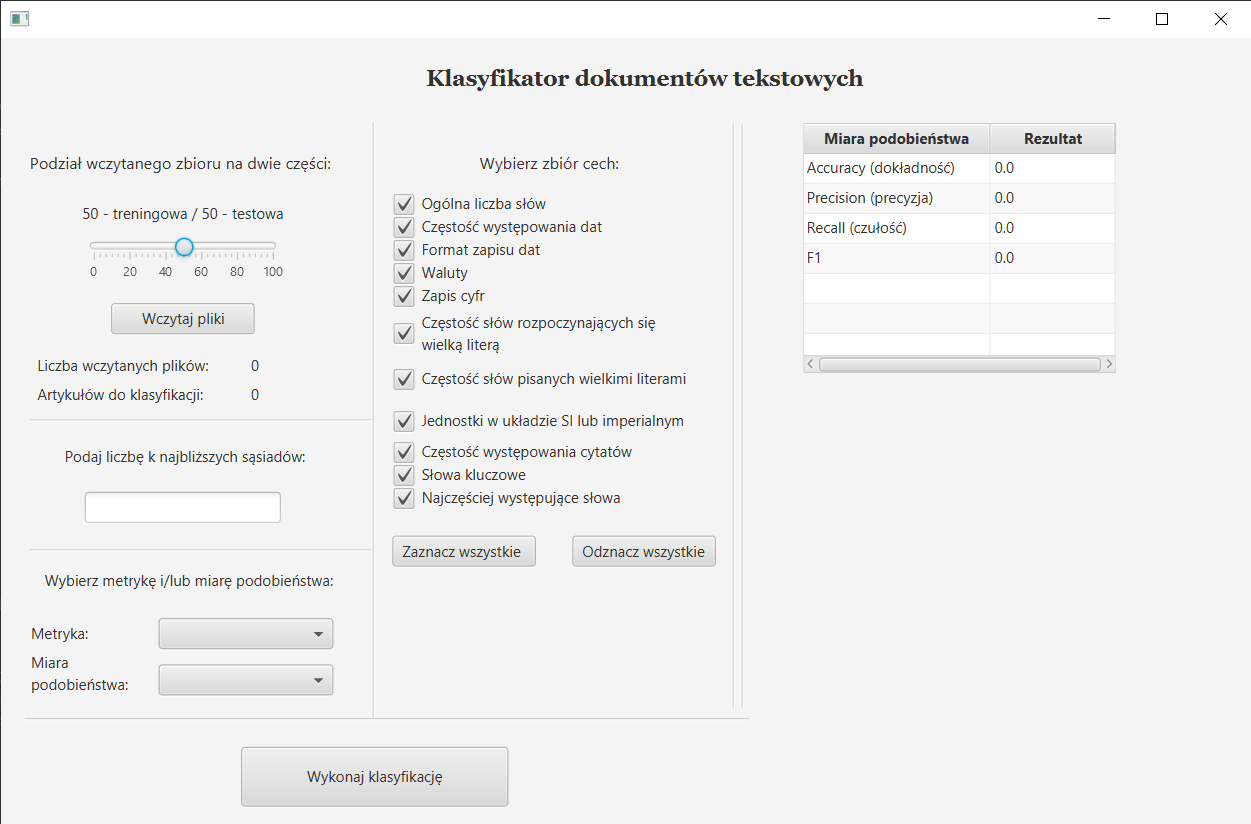
\includegraphics[width=15cm]{gui_ksr.PNG}
    \caption{Interfejs użytkownika dla aplikacji.}
\end{figure}

\section{Wyniki klasyfikacji dla różnych parametrów wejściowych}
Wyniki kolejnych eksperymentów wg punktów 2.-8. opisu projektu 1.  Wykresy i tabele
obowiązkowe, dokładnie opisane w ,,captions'' (tytułach), konieczny opis osi i
jednostek wykresów oraz kolumn i wierszy tabel.\\

{**Ewentualne wyniki realizacji punktu 9. opisu Projektu 1., czyli,,na ocenę 5.0'' i ich porównanie do wyników z
części obowiązkowej**.}\\

\noindent {\bf Sekcja uzupełniona jako efekt zadania Tydzień 05 wg Harmonogramu Zajęć
na WIKAMP KSR.}


\section{Dyskusja, wnioski}
Dokładne interpretacje uzyskanych wyników w zależności od parametrów klasyfikacji
opisanych w punktach 3.-8 opisu Projektu 1.
Szczególnie istotne są wnioski o charakterze uniwersalnym, istotne dla podobnych zadań.
Omówić i wyjaśnić napotkane problemy (jeśli były). Każdy wniosek/problem powinien mieć poparcie
w przeprowadzonych eksperymentach (odwołania do konkretnych wyników: wykresów,
tabel). \\
\underline{Dla końcowej oceny jest to najważniejsza sekcja} sprawozdania, gdyż prezentuje poziom
zrozumienia rozwiązywanego problemu.\\

** Możliwości kontynuacji prac w obszarze systemów rozpoznawania, zwłaszcza w kontekście pracy inżynierskiej,
magisterskiej, naukowej, itp. **\\

\noindent {\bf Sekcja uzupełniona jako efekt zadania Tydzień 06 wg Harmonogramu Zajęć
na WIKAMP KSR.}


\section{Braki w realizacji projektu 1.}
Wymienić wg opisu Projektu 1. wszystkie niezrealizowane obowiązkowe elementy projektu, ewentualnie
podać merytoryczne (ale nie czasowe) przyczyny tych braków.


\begin{thebibliography}{0}
\bibitem{tadeusiewicz90} R. Tadeusiewicz: Rozpoznawanie obrazów, PWN, Warszawa, 1991.
\bibitem{coca_words} Corpus of Contemporary American English: Most frequent english words [przeglądany  20.03.2021], Dostępny w: https://www.english-corpora.org/
\bibitem{reuters} Repozytorium Uniwersytety Kalifornijskiego w Irvine do nauki uczenia maszynowego: Artykuły agencji Reuters[przeglądany 20.03.2021],
Dostępny w: http://archive.ics.uci.edu/ml/machine-learning-databases/reuters21578-mld/
\bibitem{niewiadomski08} A. Niewiadomski, Methods for the Linguistic Summarization of Data: Applications of Fuzzy Sets and Their Extensions, Akademicka Oficyna Wydawnicza EXIT, Warszawa, 2008.
\bibitem{tablica_pomylek} Tablica pomyłek [przeglądany 28.03.2021], Dostępny w: https://pl.wikipedia.org/wiki/Tablica\_pomyłek
\bibitem{f1} F-score [przeglądany 28.03.2021] Dostępny w: https://en.wikipedia.org/wiki/F-score
\bibitem{wyklad} A. Niewiadomski, Materiały, przykłady i ćwiczenia do przedmiotu Komputerowe Systemy Rozpoznawania, 2020.
\bibitem{java_11} Dokumetacja Java 11 [przeglądany 11.04.2021] Dostępny w : https://docs.oracle.com/en/java/javase/11/
\bibitem{maven} Dokumentacja Maven 3.6.3 [przeglądany 11.04.2021] Dostępny w: https://maven.apache.org/docs/3.6.3/release-notes.html
\bibitem{javafx} Dokumentacja JavaFx 13 [przeglądany 11.04.2021] Dostępny w: https://openjfx.io/javadoc/13/
\end{thebibliography}

Literatura zawiera wyłącznie źródła recenzowane i/lub o potwierdzonej wiarygodności,
możliwe do weryfikacji i cytowane w sprawozdaniu.

\end{document}